\chapter{实验}
通过前面几章对MMC、MKC模型的分析,本章将使用UCI上的数据集验证模型的性能。所有实验的运行环境是MATLAB 8.6,操作系统为Windows 10,硬件环境为3.4GHz Inter Core i7处理器、8GB内存的PC上。

\section{数据集}
本次实验所使用的数据集全部来自UCI仓库,受计算资源等因素的限制,只选择了digits1v7、ionosphere和ringnorm三个数据集。数据描述如表(\ref{tab:dataset})所示:
\begin{table}[!htbp]
\caption{数据集描述}
\centering
\renewcommand\arraystretch{1.5}
\begin{tabular}{|p{3cm}<{\centering}|p{2cm}<{\centering}|p{2cm}<{\centering}|p{2cm}<{\centering}|}
\hline
数据 & 大小 & 维度 & 类别 \\
\hline 
digits1v7 & 776 & 64 & 2 \\
\hline
ionosphere & 354 & 64 & 2 \\
\hline
ringnorm & 1000 & 20 & 2 \\
\hline
\end{tabular}
\label{tab:dataset}
\end{table} 

\section{聚类精度}
首先,本文从聚类精度来验证MMC和MKC的性能。这里的聚类精度是指在最终的聚类结果中,类标记正确的数据样本个数占总数据样本数的百分比。对于MKC,这里使用了三个核函数,分别是:线性核函数$k_1(\mathbf{x}_1,\mathbf{x}_2)=\mathbf{x}_1^T\mathbf{x}_2$,多项式核函数$k_2(\mathbf{x}_1,\mathbf{x}_2)=(\mathbf{x}_1^T\mathbf{x}_2+1)^d$,高斯核函数$k_3(\mathbf{x}_1,\mathbf{x}_2)=\mathrm{exp}(-(\mathbf{x}_1-\mathbf{x}_2)^T(\mathbf{x}_1-\mathbf{x}_2)/2\sigma)$。使用iterSVM\upcite{zhang2009maximum}运行MMC算法,同时为了方便对比,本文使用k均值聚类和谱聚类作为基准。至于MKC模型中的多个参数,本文采用网格搜索,选择其使得聚类结果最优的一组参数建立模型,待搜索的参数空间见表(\ref{tab:para})。

为了评估聚类精度,本文采用的策略是:首先采用有类标记的数据集,去掉所有的类标记并运行聚类算法,然后将聚类得到的结果与类标记进行对比,计算聚类精度。依据此策略,实验最终运行得到的聚类结果见表(\ref{tab:result})。
\begin{table}[!htbp]
\caption{MKC的参数空间}
\centering
\small
\renewcommand\arraystretch{1.5}
\begin{tabular}{p{1.5cm}<{\centering}|p{12cm}}
\hline
参数 & \hspace{0.5cm}取值空间\\
\hline
$C$ &  \hspace{0.5cm}$2^{-6} \quad 2^{-5} \quad 2^{-4} \quad 2^{-3} \quad 2^{-2} \quad 2^{-1} \quad 2^{0} \quad 2^{1} \quad 2^{2} \quad 2^{3} \quad 2^{4} \quad 2^{5} \quad 2^{6} $\\
\hline
$d$ &  \hspace{0.5cm}$2^{0} \quad 2^{1} \quad 2^{2} \quad 2^{3} \quad 2^{4} \quad 2^{5} \quad 2^{6} \quad 2^{7} \quad 2^{8} \quad 2^{9} \quad 2^{10}$ \\
\hline
$\sigma$ &  \hspace{0.5cm}$0.5 \quad 1 \quad 2 \quad 5 \quad 7 \quad 10 \quad 12 \quad 15 \quad 17 \quad 20 $\\
\hline
\end{tabular}
\label{tab:para}
\end{table} 

\begin{table}[!htbp]
\caption{聚类精度(\%)}
\centering
\small
\renewcommand\arraystretch{1.5}
\begin{tabular}{|p{2cm}<{\centering}|p{1.3cm}<{\centering}|p{1.3cm}<{\centering}|p{1.3cm}<{\centering}|p{1.3cm}<{\centering}|p{1.3cm}<{\centering}|p{1.3cm}<{\centering}|p{1.3cm}<{\centering}|}
\hline
数据 & $K_1$ & $K_2$ & $K_3$ & MKC & iterSVM & KM & PC \\
\hline
digits1v7 & 99.61 & 99.61 & 97.62 & 99.74 & 99.36 & 99.23 & 50.26 \\
\hline
ionosphere & 77.78 & 81.48 & 78.06 & 87.46 & 63.84 & 71.23 & 72.60 \\
\hline
ringnorm & 74.50 & 96.90 & 98.70 & 96.50 & 79.11 & 75.55 & 92.27 \\
\hline
\end{tabular}
\label{tab:result}
\end{table}

从表(\ref{tab:result})可以看出,MKC算法的聚类精度确实比MMC、k均值和谱聚类高。在digits1v7、ionosphere和ringnorm三个数据集中,k均值和谱聚类的精度明显受到数据集内部结构的影响,存在忽高忽低的情况。而MKC相比较k均值和谱聚类而言,其聚类结果更加稳定,而且受到数据集内部结构的影响程度不大。但是从图(\ref{fig:ionosphere-gpm})、(\ref{fig:digits1v7-gpm})和(\ref{fig:ringnorm-gpm})可以看出,MKC算法在割平面迭代过程中,其聚类精度是十分不稳定的。随着迭代次数的增加,其聚类精度呈现出上下跳跃的状态,因此,即使割平面最终收敛,但得到的模型的聚类精度可能并不高。所以本文以割平面过程中使得聚类精度最高的参数生成MKC模型,而非最终迭代终止时的参数。

\begin{figure}[H]
  \centering
  \begin{minipage}[t]{0.45\linewidth}
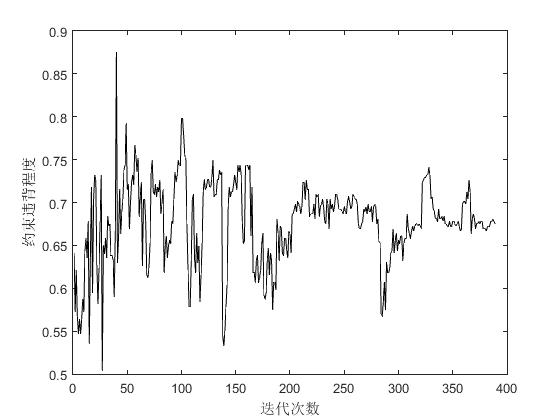
\includegraphics[width=\textwidth]{figure/ionosphere_acc.jpg}
  \caption{ionosphere割平面收敛过程}
  \label{fig:ionosphere-gpm}
  \end{minipage}
  \begin{minipage}[t]{0.45\linewidth}
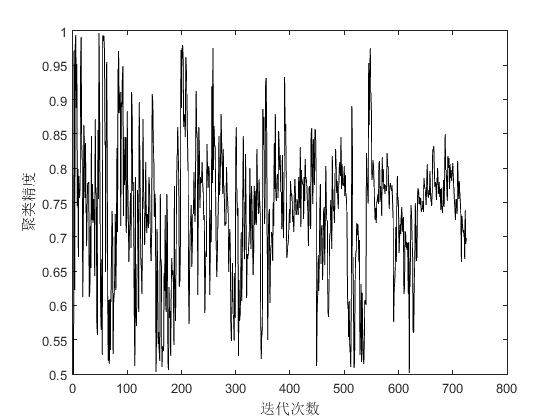
\includegraphics[width=\textwidth]{figure/digits1v7_acc.jpg}
  \caption{digits1v7割平面收敛过程}
  \label{fig:digits1v7-gpm}
  \end{minipage}
  \begin{minipage}[t]{0.45\linewidth}
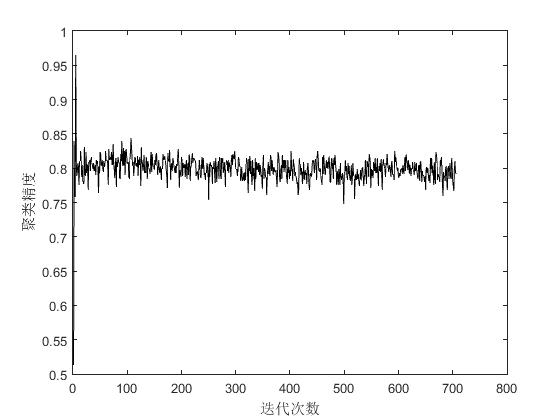
\includegraphics[width=\textwidth]{figure/ringnorm_acc.jpg}
  \caption{ringnorm割平面收敛过程}
  \label{fig:ringnorm-gpm}
  \end{minipage}
\end{figure}



\section{速度}
关于MKC的潜在担忧可能是时间复杂度问题。显然,MKC算法中割平面过程的收敛时间由数据规模和终止条件$\epsilon$共同决定。因此论文从这两个方面进行了相关实验,并将结果进行图形化展示。从图(\ref{fig:time})可以看出,随着数据规模的增大,MKC算法的收敛时间随着终止条件$\epsilon$的减小而迅速增大,甚至在有限的时间内无法收敛。另外从图(\ref{fig:ionosphere-xi})、(\ref{fig:digits1v7-xi})和(\ref{fig:ringnorm-xi})可以看到,MKC的割平面过程收敛十分缓慢,并且存在上下波动的情况,但其总体趋势是下降的,这也符合割平面方法的思想。

\begin{figure}[H]
  \centering
  \begin{minipage}[t]{0.45\linewidth}
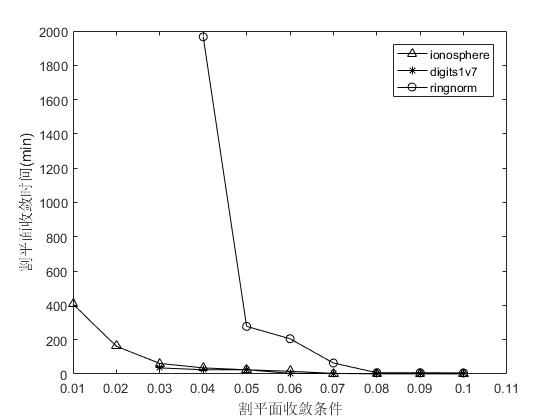
\includegraphics[width=\textwidth]{figure/time.jpg}
  \caption{MKC算法的收敛情况}
  \label{fig:time}
  \end{minipage}
  \begin{minipage}[t]{0.45\linewidth}
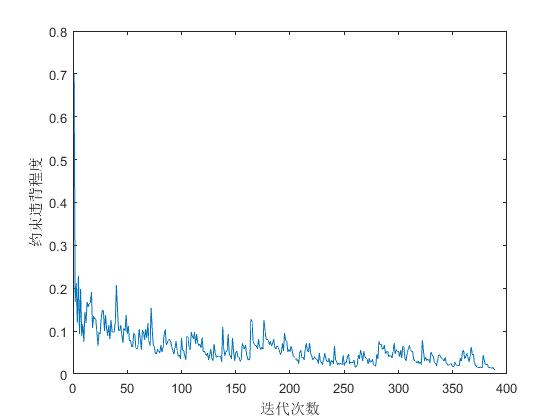
\includegraphics[width=\textwidth]{figure/ionosphere_xi.jpg}
  \caption{ionosphere割平面收敛过程}
  \label{fig:ionosphere-xi}
  \end{minipage}
  \begin{minipage}[t]{0.45\linewidth}
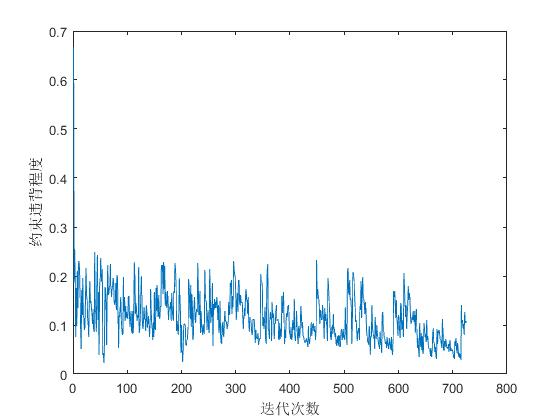
\includegraphics[width=\textwidth]{figure/digits1v7_xi.jpg}
  \caption{digits1v7割平面收敛过程}
  \label{fig:digits1v7-xi}
  \end{minipage}
  \begin{minipage}[t]{0.45\linewidth}
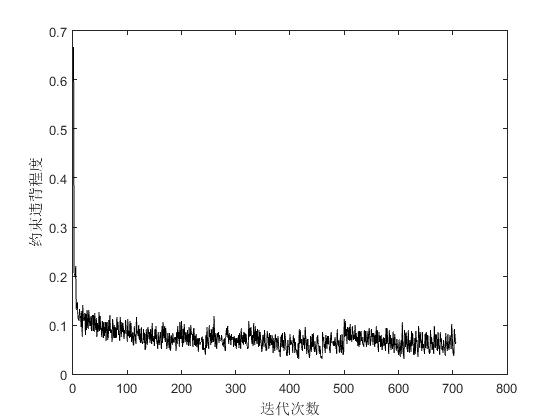
\includegraphics[width=\textwidth]{figure/ringnorm_xi.jpg}
  \caption{ringnorm割平面收敛过程}
  \label{fig:ringnorm-xi}
  \end{minipage}
\end{figure}

\section{泛化能力}
MKC采用了SVM中的间隔最大化学习策略,因此本文实验也测试了MKC在未知数据上的泛化能力。首先从总数据集上随机获取一定规模的子集作为训练数据集,剩下的数据集作为测试数据集。然后利用训练数据集学习得到MKC模型,并使用此模型在测试数据集上进行聚类。
\begin{table}[!htbp]
\caption{MKC的泛化能力(\%)}
\centering
\small
\renewcommand\arraystretch{1.5}
\begin{tabular}{|p{2cm}<{\centering}|p{2.5cm}<{\centering}|p{2.5cm}<{\centering}|}
\hline
数据 & 训练数据集 & 测试数据集 \\
\hline
digits1v7 & 99.74 & 98.92 \\
\hline
ringnorm & 87.46 & 87.19  \\
\hline
\end{tabular}
\label{tab:generalize}
\end{table} 

观察表(\ref{tab:generalize}),发现对数据集的子集进行训练得到的模型在测试数据集上也能取得较好的效果,也即泛化性能较好。受这个结果的启发,在对数据集进行学习训练过程中,若数据集规模较大,可以以一定的策略(比如随机)选择数据集的一个小的子集作为训练集,再在这个训练集上进行训练,得到的MKC模型在整个数据集上同样能得到很好的聚类效果。

\section{本章小结}
本章使用UCI上的数据集进行实验来验证MKC模型的性能,并与传统的k均值聚类和谱聚类进行比较。从前面的实验可以看出,与传统的k均值和谱聚类相比,MKC算法的聚类精度较高,较好的克服了数据集内部结构对模型聚类精度的影响。但MKC模型的训练过程需要较长的时间,并且其割平面迭代过程很不稳定,每轮割平面得到的模型进行聚类时,得到的精确度跳跃特别大,上下剧烈抖动,造成割平面收敛时得到的模型不一定是最优的,本文以迭代过程中聚类精度最高的参数作为最优模型的参数。此外,MKC算法具有较好的泛化性能,这使得MKC算法能轻松应对大规模数据集。